\documentclass[]{standalone}
\usepackage{tikz}
\usepackage{pgffor}

\standaloneenv{tikzpicture}

\usetikzlibrary{arrows}

\newcommand\colorWorldlayer{black}
\newcommand\colorLightcone{blue}
\newcommand\colorWorldline{red}
\newcommand\colorWorldlineII{green}

\newcommand\worldlineLength{5}
\newcommand\worldlineN{5}
\newcommand\worldlineDist{0.5}

\newcommand\drawWorldlines{
	\foreach \i in {0,...,\worldlineN}{	
		\draw[color=\colorWorldlayer] (0,\i*\worldlineDist) to (\worldlineLength,\i*\worldlineDist);
	}
}

\newcommand\drawWorldlayers{
	\foreach \i in {0,...,\worldlineN}{	
		\draw[color=\colorWorldlayer]
		(\worldlineDist,\i*\worldlineDist+\worldlineDist) to
		++(-\worldlineDist, -\worldlineDist) to
		++(\worldlineLength,0) to
		++(\worldlineDist, \worldlineDist);
	}
}

\newcommand\drawWorldlayersLabels{
	\foreach \i in {0,...,\worldlineN}{	
		\draw (-0.75, \i*\worldlineDist+0.2) node[anchor=east](){$t=\i$};
	}
}

\begin{document}
	
	
	%% output-name: gleichzeitebenen
	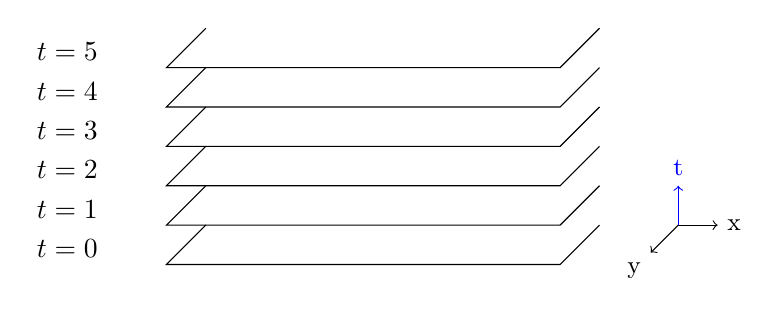
\begin{tikzpicture}
		
		\newcommand\coordinateSystemPosX{6.5}
		\newcommand\coordinateSystemPosY{0.5}
		\newcommand\coordinateSystemColX{black}
		\newcommand\coordinateSystemColY{black}
		\newcommand\coordinateSystemColT{blue}
		\newcommand\coordinateSystemArrowLen{0.5}
		
		\drawWorldlayers
		\drawWorldlayersLabels
	
		\draw[->, color=\coordinateSystemColX] (\coordinateSystemPosX, \coordinateSystemPosY) to ++(\coordinateSystemArrowLen, 0) node[anchor=west](){\small x};
		\draw[->, color=\coordinateSystemColY] (\coordinateSystemPosX, \coordinateSystemPosY) to ++(-\coordinateSystemArrowLen*0.7, -\coordinateSystemArrowLen*0.7) node[anchor=north east](){\small y};
		\draw[->, color=\coordinateSystemColT] (\coordinateSystemPosX, \coordinateSystemPosY) to ++(0, \coordinateSystemArrowLen) node[anchor=south](){\small t};
	\end{tikzpicture}
	
	%% output-name: weltlinien_3d
	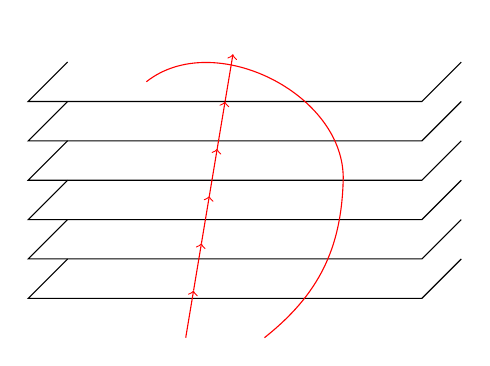
\begin{tikzpicture}
		\drawWorldlayers
		
		\newcommand\wlDX{0.1}
		\newcommand\wlDY{0.6}
		\foreach \i in {0,...,\worldlineN}{	
			\draw[->, color=\colorWorldline] (2+\wlDX*\i,-0.5+\wlDY*\i) to ++(\wlDX, \wlDY);
		}
	
		\draw[color=\colorWorldline]
			(3,-0.5)
			to[smooth, bend right=25] (4,1.5)
			%to[smooth, bend right=45] (3.75,1.7)
			to[smooth, bend right =65] (1.5,2.75);
	\end{tikzpicture}

	%% output-name: gleichgeschwindigkeitskegel
	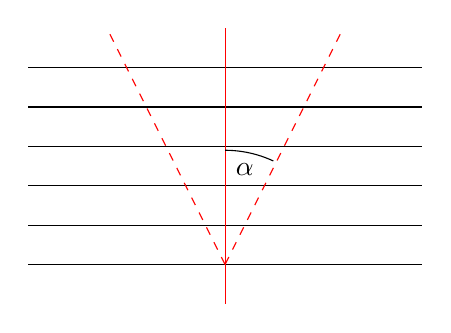
\begin{tikzpicture}
		\drawWorldlines
	
		\draw[color=\colorWorldline] (2.5,-0.5) to (2.5, 3);
		\draw[color=\colorWorldline, dashed] (2.5,0) to (1, 3);
		\draw[color=\colorWorldline, dashed] (2.5,0) to (4, 3);
		\draw[] (2.5,1.45) arc (90:65:1.45);
		\node at (2.75,1.2){$\alpha$};
	\end{tikzpicture}
	
	%% output-name: lichtkegel
	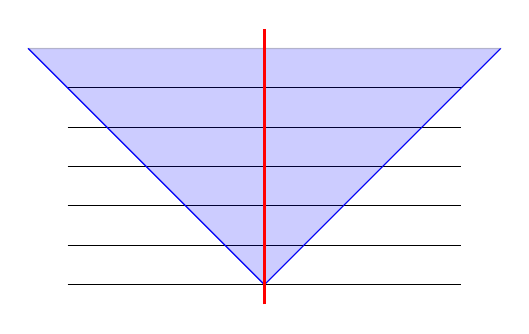
\begin{tikzpicture}
	\drawWorldlines
	
	\newcommand\lightconePosX{2.5}
	\newcommand\lightconePosY{0}
	\newcommand\lightconeHeight{3}
	\newcommand\lightconeHalfWidth{3}
	\newcommand\lightconeOpacity{0.2}
	
	\draw[fill=\colorLightcone, opacity=\lightconeOpacity]
	(\lightconePosX, \lightconePosY) to
	++(-\lightconeHalfWidth, \lightconeHeight) to
	++(+2*\lightconeHalfWidth, 0) to
	cycle;
	\draw[color=\colorLightcone]
	(\lightconePosX, \lightconePosY) to
	++(-\lightconeHalfWidth, \lightconeHeight);
	\draw[color=\colorLightcone]
	(\lightconePosX, \lightconePosY) to
	++(\lightconeHalfWidth, \lightconeHeight);
	
	\draw[color=\colorWorldline, thick] (\lightconePosX, \lightconePosY-0.25) to ++(0,3.5);
	\end{tikzpicture}
	
	%% output-name: lichtkegel_beobachter_klassisch
	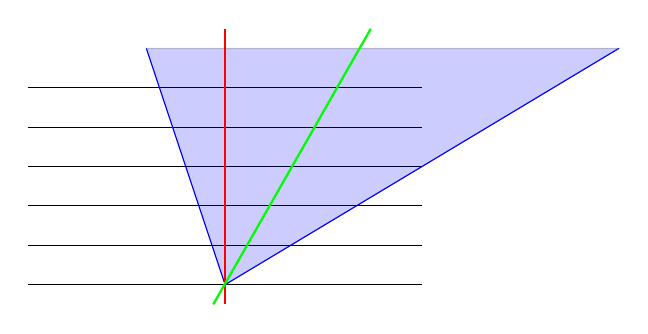
\begin{tikzpicture}
	\drawWorldlines
	
	\newcommand\lightconePosX{2.5}
	\newcommand\lightconePosY{0}
	\newcommand\lightconeHeight{3}
	\newcommand\lightconeHalfWidth{3}
	\newcommand\lightconeOpacity{0.2}
	
	\newcommand\lightconeShift{2}
	
	\draw[fill=\colorLightcone, opacity=\lightconeOpacity]
	(\lightconePosX, \lightconePosY) to
	++(-\lightconeHalfWidth+\lightconeShift, \lightconeHeight) to
	++(+2*\lightconeHalfWidth, 0) to
	cycle;
	\draw[color=\colorLightcone]
	(\lightconePosX, \lightconePosY) to
	++(-\lightconeHalfWidth+\lightconeShift, \lightconeHeight);
	\draw[color=\colorLightcone]
	(\lightconePosX, \lightconePosY) to
	++(\lightconeHalfWidth+\lightconeShift, \lightconeHeight);
	
	\draw[color=\colorWorldline, thick] (\lightconePosX, \lightconePosY-0.25) to ++(0,3.5);
	\draw[color=\colorWorldlineII, thick] (\lightconePosX-0.15, \lightconePosY-0.25) to ++(\lightconeShift,3.5);
	\end{tikzpicture}
	
	%% output-name: lichtkegel_beobachter_relativistisch
	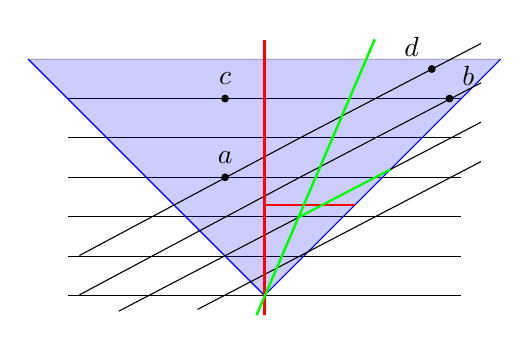
\begin{tikzpicture}
		\drawWorldlines
		
		\newcommand\lightconePosX{2.5}
		\newcommand\lightconePosY{0}
		\newcommand\lightconeHeight{3}
		\newcommand\lightconeHalfWidth{3}
		\newcommand\lightconeOpacity{0.2}
		
		\draw[fill=\colorLightcone, opacity=\lightconeOpacity]
			(\lightconePosX, \lightconePosY) to
			++(-\lightconeHalfWidth, \lightconeHeight) to
			++(+2*\lightconeHalfWidth, 0) to
			cycle;
		\draw[color=\colorLightcone]
			(\lightconePosX, \lightconePosY) to
			++(-\lightconeHalfWidth, \lightconeHeight);
		\draw[color=\colorLightcone]
			(\lightconePosX, \lightconePosY) to
			++(\lightconeHalfWidth, \lightconeHeight);
			
		\draw[color=\colorWorldline, thick] (\lightconePosX, \lightconePosY-0.25) to ++(0,3.5);
		\draw[color=\colorWorldlineII, thick] (\lightconePosX-0.1, \lightconePosY-0.25) to ++(1.5,3.5);
		
		\draw[] (2.95,1-0.5) to ++(+2.30,+1.2);
		\draw[] (2.95,1-0.5) to ++(-1.3,-0.678);
		
		\draw[] (2.95,1) to ++(+2.30,+1.2);
		\draw[] (2.95,1) to ++(-2.30,-1.2);
		
		\draw[] (2.95,1+0.5) to ++(+2.30,+1.2);
		\draw[] (2.95,1+0.5) to ++(-2.80,-1.493);
		
		\draw[] (2.95,1+1.0) to ++(+2.30,+1.2);
		\draw[] (2.95,1+1.0) to ++(-2.80,-1.493);
		
		\draw[color=\colorWorldline, thick] (\lightconePosX, \lightconePosY-0.25) to ++(0,3.5);
		\draw[color=\colorWorldline, thick] (2.5,1.15) to ++(1.15,0);
		\draw[color=\colorWorldlineII, thick] (\lightconePosX-0.1, \lightconePosY-0.25) to ++(1.5,3.5);
		\draw[color=\colorWorldlineII, thick] (2.95,1) to ++(1.15,0.6);
		
		\node[circle,fill,inner sep=1pt, label=above:$a$] at (2.0,1.5) {};
		\node[circle,fill,inner sep=1pt, label=above:$c$] at (2.0,2.5) {};
		\node[circle,fill,inner sep=1pt, label=above right:$b$] at (4.85,2.5) {};
		\node[circle,fill,inner sep=1pt, label=above left:$d$] at (4.625,2.875) {};
	\end{tikzpicture}
	
	%% output-name: poincare
	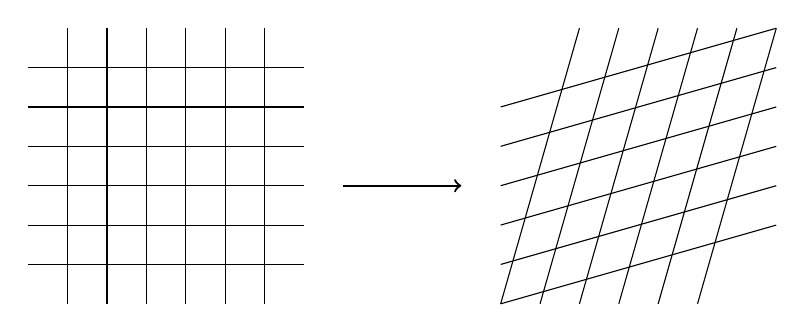
\begin{tikzpicture}
		\foreach \i in {0,...,5}{	
			\draw[color=\colorWorldlayer] (0,\i*0.5) to (3.5,\i*0.5);
		}
	
		\foreach \i in {1,...,6}{	
			\draw[color=\colorWorldlayer] (\i*0.5,-0.5) to (\i*0.5,3);
		}
	
		\draw[->, thick] (4,1) -- (5.5,1);
	
		\foreach \i in {0,...,5}{	
			\draw[color=\colorWorldlayer] (0+6,\i*0.5-0.5) to (3.5+6,\i*0.5+0.5);
		}
		
		\foreach \i in {1,...,6}{	
			\draw[color=\colorWorldlayer] (\i*0.5-0.5+6,-0.5) to (\i*0.5+0.5+6,3);
		}
	\end{tikzpicture}
	
	%% output-name: geodaeten
	\begin{tikzpicture}
		\node[rectangle, inner sep=50pt, draw] at (0,0) {};
		\node[circle, fill, inner sep=1pt, label=left:A] (a1) at (-0.6,-1) {};
		\node[circle, fill, inner sep=1pt, label=above:B] (b1) at (1.2,0.9) {};
		\draw[] (a1) -- (b1); 
		
		\node[circle,    inner sep=40pt, draw] at (6,0) {};
		\node[circle, fill, inner sep=1pt, label=below:A] (a2) at (4.7,0) {};
		\node[circle, fill, inner sep=1pt, label=above:B] (b2) at (7,1.1) {};
		\draw[] (a2) to[bend left=15] (b2); 
		\draw[dashed] (a2) to (b2); 		
		
	\end{tikzpicture}
	
	%% output-name: gravitation
	\begin{tikzpicture}
		\node[rectangle, inner sep=50pt, draw] at (0,0) {};
		\draw[] (-0.25,-1.25) -- ++(0,2.5); 
		\draw[] (+0.25,-1.25) -- ++(0,2.5); 
		
		\node[circle,    inner sep=40pt, draw] at (6,0) {};
		\draw[dashed] (4,0) to[bend right=10] (8,0); 	
		\draw[] (5.75,-0.2) to[bend left=5] (6,2); 	
		\draw[] (6.25,-0.2) to[bend right=5] (6,2); 	
	\end{tikzpicture}
	
	%% output-name: lichtkegel_gekippt
	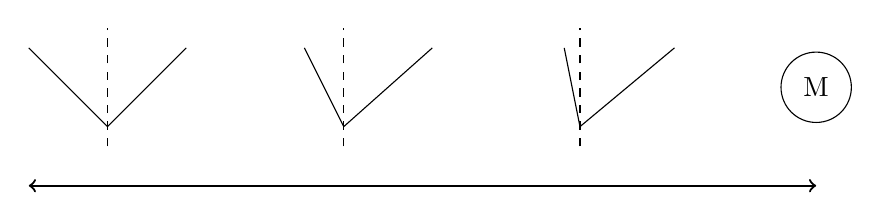
\begin{tikzpicture}
		\newcommand\tiltedlightcone[2]{ %% argument 1: x-position, argument 2: shift
			\draw (#1,0.5) -- ++(-1+#2,1);
			\draw (#1,0.5) -- ++(+1+0.25*#2,1);
			\draw[dashed] (#1,0.25) -- (#1,1.75);
		}	
	
		\draw[<->, thick] (0,-0.25) -- ++(10,0);
	
		\tiltedlightcone{1}{0}
		\tiltedlightcone{4}{0.5}
		\tiltedlightcone{7}{0.8}
		
		\node[circle, inner sep=5pt, draw] at (10,1){M};
	\end{tikzpicture}
	
	%% output-name: schwarzes_loch
	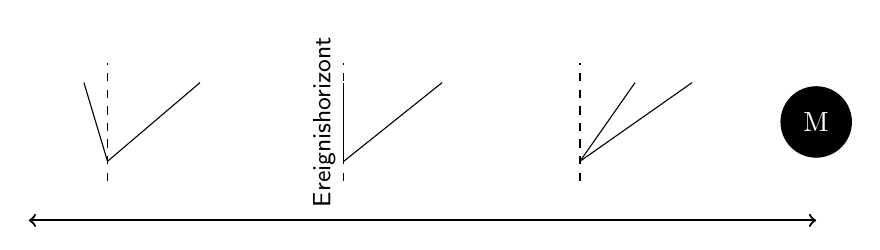
\begin{tikzpicture}
		\newcommand\tiltedlightcone[2]{ %% argument 1: x-position, argument 2: shift
			\draw (#1,0.5) -- ++(-1+#2,1);
			\draw (#1,0.5) -- ++(+1+0.25*#2,1);
			\draw[dashed] (#1,0.25) -- (#1,1.75);
		}	
		
		\draw[<->, thick] (0,-0.25) -- ++(10,0);
		
		\tiltedlightcone{1}{0.7}
		\tiltedlightcone{4}{1}
		\tiltedlightcone{7}{1.7}
		
		\node[circle, inner sep=5pt, draw, fill] at (10,1){\textcolor{white}{M}};
		
		\node[rotate=90] at (3.75,1) {\small\textsf{Ereignishorizont}};
	\end{tikzpicture}

\end{document}